\documentclass[journal,12pt,twocolumn]{IEEEtran}

\usepackage{setspace}
\usepackage{gensymb}
\singlespacing
\usepackage[cmex10]{amsmath}

\usepackage{amsthm}

\usepackage{mathrsfs}
\usepackage{txfonts}
\usepackage{stfloats}
\usepackage{bm}
\usepackage{cite}
\usepackage{cases}
\usepackage{subfig}

\usepackage{longtable}
\usepackage{multirow}

\usepackage{enumitem}
\usepackage{mathtools}
\usepackage{steinmetz}
\usepackage{tikz}
\usepackage{circuitikz}
\usepackage{verbatim}
\usepackage{tfrupee}
\usepackage[breaklinks=true]{hyperref}
\usepackage{graphicx}
\usepackage{tkz-euclide}

\usetikzlibrary{calc,math}
\usepackage{listings}
    \usepackage{color}                                            %%
    \usepackage{array}                                            %%
    \usepackage{longtable}                                        %%
    \usepackage{calc}                                             %%
    \usepackage{multirow}                                         %%
    \usepackage{hhline}                                           %%
    \usepackage{ifthen}                                           %%
    \usepackage{lscape}     
\usepackage{multicol}
\usepackage{chngcntr}

\DeclareMathOperator*{\Res}{Res}

\renewcommand\thesection{\arabic{section}}
\renewcommand\thesubsection{\thesection.\arabic{subsection}}
\renewcommand\thesubsubsection{\thesubsection.\arabic{subsubsection}}

\renewcommand\thesectiondis{\arabic{section}}
\renewcommand\thesubsectiondis{\thesectiondis.\arabic{subsection}}
\renewcommand\thesubsubsectiondis{\thesubsectiondis.\arabic{subsubsection}}


\hyphenation{op-tical net-works semi-conduc-tor}
\def\inputGnumericTable{}                                 %%

\lstset{
%language=C,
frame=single, 
breaklines=true,
columns=fullflexible
}
\begin{document}


\newtheorem{theorem}{Theorem}[section]
\newtheorem{problem}{Problem}
\newtheorem{proposition}{Proposition}[section]
\newtheorem{lemma}{Lemma}[section]
\newtheorem{corollary}[theorem]{Corollary}
\newtheorem{example}{Example}[section]
\newtheorem{definition}[problem]{Definition}

\newcommand{\BEQA}{\begin{eqnarray}}
\newcommand{\EEQA}{\end{eqnarray}}
\newcommand{\define}{\stackrel{\triangle}{=}}
\bibliographystyle{IEEEtran}
\raggedbottom
\setlength{\parindent}{0pt}
\providecommand{\mbf}{\mathbf}
\providecommand{\pr}[1]{\ensuremath{\Pr\left(#1\right)}}
\providecommand{\qfunc}[1]{\ensuremath{Q\left(#1\right)}}
\providecommand{\sbrak}[1]{\ensuremath{{}\left[#1\right]}}
\providecommand{\lsbrak}[1]{\ensuremath{{}\left[#1\right.}}
\providecommand{\rsbrak}[1]{\ensuremath{{}\left.#1\right]}}
\providecommand{\brak}[1]{\ensuremath{\left(#1\right)}}
\providecommand{\lbrak}[1]{\ensuremath{\left(#1\right.}}
\providecommand{\rbrak}[1]{\ensuremath{\left.#1\right)}}
\providecommand{\cbrak}[1]{\ensuremath{\left\{#1\right\}}}
\providecommand{\lcbrak}[1]{\ensuremath{\left\{#1\right.}}
\providecommand{\rcbrak}[1]{\ensuremath{\left.#1\right\}}}
\theoremstyle{remark}
\newtheorem{rem}{Remark}
\newcommand{\sgn}{\mathop{\mathrm{sgn}}}
\providecommand{\abs}[1]{\left\vert#1\right\vert}
\providecommand{\res}[1]{\Res\displaylimits_{#1}} 
\providecommand{\norm}[1]{\left\lVert#1\right\rVert}
%\providecommand{\norm}[1]{\lVert#1\rVert}
\providecommand{\mtx}[1]{\mathbf{#1}}
\providecommand{\mean}[1]{E\left[ #1 \right]}
\providecommand{\fourier}{\overset{\mathcal{F}}{ \rightleftharpoons}}
%\providecommand{\hilbert}{\overset{\mathcal{H}}{ \rightleftharpoons}}
\providecommand{\system}{\overset{\mathcal{H}}{ \longleftrightarrow}}
	%\newcommand{\solution}[2]{\textbf{Solution:}{#1}}
\newcommand{\solution}{\noindent \textbf{Solution: }}
\newcommand{\cosec}{\,\text{cosec}\,}
\providecommand{\dec}[2]{\ensuremath{\overset{#1}{\underset{#2}{\gtrless}}}}
\newcommand{\myvec}[1]{\ensuremath{\begin{pmatrix}#1\end{pmatrix}}}
\newcommand{\mydet}[1]{\ensuremath{\begin{vmatrix}#1\end{vmatrix}}}
\numberwithin{equation}{subsection}
\makeatletter
\@addtoreset{figure}{problem}
\makeatother
\let\StandardTheFigure\thefigure
\let\vec\mathbf
\renewcommand{\thefigure}{\theproblem}
\def\putbox#1#2#3{\makebox[0in][l]{\makebox[#1][l]{}\raisebox{\baselineskip}[0in][0in]{\raisebox{#2}[0in][0in]{#3}}}}
     \def\rightbox#1{\makebox[0in][r]{#1}}
     \def\centbox#1{\makebox[0in]{#1}}
     \def\topbox#1{\raisebox{-\baselineskip}[0in][0in]{#1}}
     \def\midbox#1{\raisebox{-0.5\baselineskip}[0in][0in]{#1}}
\vspace{3cm}
\title{EE3025 ASSIGNMENT- 1}
\author{Mohammed Sadiq - EE18BTECH11051}
\maketitle
\newpage
\bigskip
\renewcommand{\thefigure}{\theenumi}
\renewcommand{\thetable}{\theenumi}
Download all python codes from 
\begin{lstlisting}
https://github.com/Sadiq0123/EE3025-IDP/tree/main/Assignment-1/codes
\end{lstlisting}
And Latex-tikz codes from - 
\begin{lstlisting}
https://github.com/Sadiq0123/EE3025-IDP/tree/main/Assignment-1
\end{lstlisting}
%
\section{\textbf{Problem}}
    
Modify the following code given in problem 2.3 with different input parameters to get the best possible output.
\begin{lstlisting}
import soundfile as sf
from scipy import signal
    
#read .wav file
input_signal,fs = sf.read('Sound_Noise.wav')
    
#sampling frequency of Input signal
sampl_freq=fs
    
#order of the filter
order = 3
    
#cutoff frequency 4kHz
cutoff_freq=4000.0
    
#digital frequency
Wn=2*cutoff_freq/sampl_freq
    
# b and a are numerator and denominator polynomials respectively
b, a = signal.butter(order,Wn,'low')
    
#filter the input signal with butterworth filter
output_signal = signal.filtfilt(b, a, input_signal)
#output_signal = signal.lfilter(b, a, input_signal)
    
#write the output signal into .wav file
sf.write('Sound_With_ReducedNoise.wav', output_signal, fs)
    
\end{lstlisting}

  \section{\textbf{Solution}}
  As we can see in the code, the input parameters that can be modified are:
  \begin{description}[font=$\bullet$\scshape\bfseries]
  \item[]{Order of the filter}
  \item[]{Cutoff frequency}
  \item[]{Function for applying the filter}
  \end{description}
  
  \subsection{\textbf{Order of the Butterworth filter}}
  As we know that higher the order of the butterworth filter, steeper will be it's fall off rate. The figure \ref{fig:Figure1} plots the amplitude response for different orders of butterworth low pass filter. 

\begin{figure}[!h]
\centering
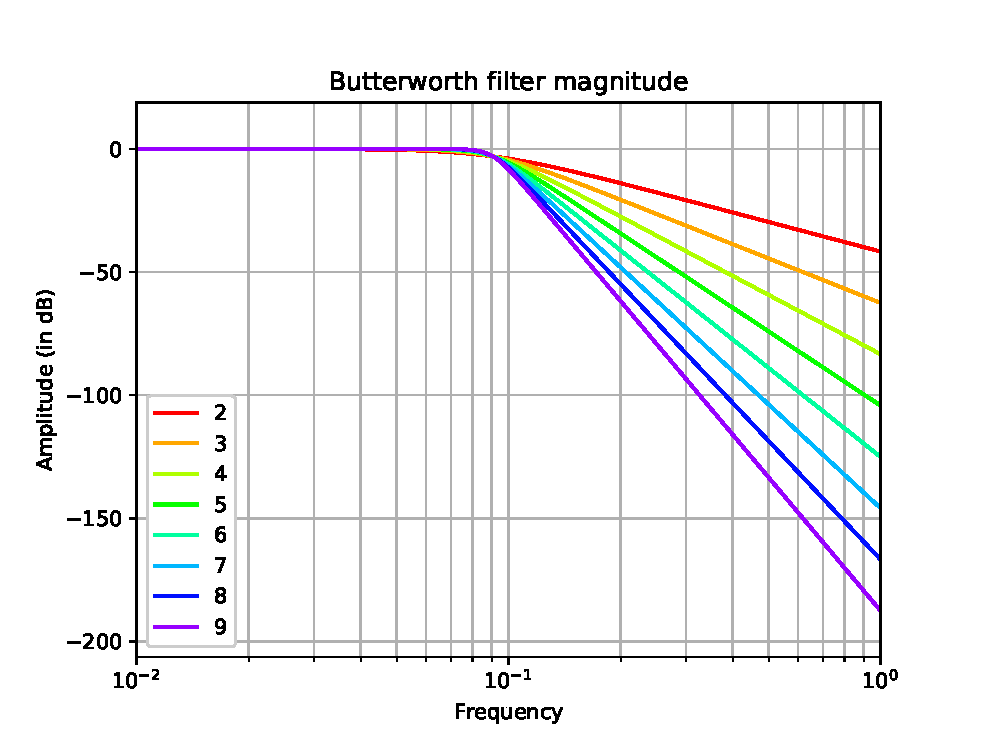
\includegraphics[width=1.2\columnwidth]{./figs/ee18btech11051_1.eps}
\caption{Filter order Magnitude response}
\label{fig:Figure0}
\end{figure}


It would look like simply increasing the order of the filter would give better results. But higher order filters are unstable when simulating. This is because the values of coefficients of numerator go below the single-precision of float numbers as order increases. At order 4, the values of coefficients of numerator are $10^{-3}$. Whereas at order 10, the order of values is $10^{-8}$. This makes it clear that we can't simply select a very high order to filter out all the noise. As we know that the transfer function for an N order filter is:
\begin{align}
\label{eq:Butterworth}
    H\brak{\j\omega} = \frac{1}{\sqrt{1+\brak{\frac{\omega}{\omega_{c}}}^{2N}}}
\end{align} 
As very high order filter is not possible, we can apply the more accurate lower order filter multiple times for better noise filtering. Now we try to establish that these two are essentially the same. Response for an order of 2N would be:
\begin{align}
\label{eq:B_high}
    |H\brak{\j\omega}| = \frac{1}{\sqrt{1+\brak{\frac{\omega}{\omega_{c}}}^{2*2N}}}
\end{align} 
\begin{align}
\label{eq:B_high2}
   |H\brak{\j\omega}|_{in dB} = -10\log_{10}\brak{1+\brak{\frac{\omega}{\omega_{c}}}^{4N}}
\end{align} 
\begin{align}
\label{eq:B_high3}
    At \frac{\omega}{\omega_{c}}>>1, |H\brak{\j\omega}|_{in dB} = -40N\log_{10}\brak{\frac{\omega}{\omega_{c}}}
\end{align} 

Now doing the same for an order N filter, but applying it twice we get:
\begin{align}
\label{eq:B_low}
    |H\brak{\j\omega}| = \brak{\frac{1}{\sqrt{1+\brak{\frac{\omega}{\omega_{c}}}^{2N}}}}^2
\end{align} 
\begin{align}
\label{eq:B_low2}
   |H\brak{\j\omega}|_{in dB} = -20\log_{10}\brak{1+\brak{\frac{\omega}{\omega_{c}}}^{2N}}
\end{align} 
\begin{align}
\label{eq:B_low3}
    At \frac{\omega}{\omega_{c}}>>1, |H\brak{\j\omega}|_{in dB} = -40N\log_{10}\brak{\frac{\omega}{\omega_{c}}}
\end{align} 

Clearly from \ref{eq:B_high3} and \ref{eq:B_low3}, applying a low order filter twice gives the same result as the filter with double the order.


  \subsection{\textbf{Cutoff frequency}}
  To get better noise filtering, we also need to tweak the cutoff frequency. One method of doing this is to locate the location of all the peaks in the frequency magnitude plot, and choose the frequency at which the last peak occurs that has height above a fixed threshold. For the given soundfile, a threshold of 500 gives the last frequency with a peak as 2111. So, we filter all the frequency components above 2111 Hz.
  
  \subsection{\textbf{Function for applying the filter}}
  The code has 2 options for applying the filter \textbf{signal.filtfilt} and \textbf{signal.lfilter}. The latter function just passes the array through the butterworth filter. Doing so introduces a phase shift of $-\pi/2$. Whereas \textbf{signal.filtfilt} does more than that. It is actually a forward-backward filter(i.e. after applying the filter once, it reverses the signal and passes it through the filter once again). This helps cancel the phase shift caused earlier. So to get best results, we can apply \textbf{signal.filtfilt} more than once.
  \\
  
  But there is one big drawback to using the forward-backward filter. That is that it is not causal. So, it can only be used on recorded signals that are already complete. For real-time filtering like in case of phone calls, we have no choice but to use \textbf{signal.lfilter} which injects a phase shift.
  \\~\\
  
  The code used for plotting the filter response and printing the coefficients can be found at- 
  \begin{lstlisting}
https://github.com/Sadiq0123/EE3025-IDP/tree/main/Assignment-1/codes/generate_plot.py
  \end{lstlisting}
  
  The soundfile generated from this algorithm can be found at - 
  \begin{lstlisting}
https://github.com/Sadiq0123/EE3025-IDP/tree/main/Assignment-1/soundfiles/Sound_optimized.wav
  \end{lstlisting}
  

\section{\textbf{Results}}
To verify that the new parameters have filtered the signal, we plot the frequency response and time-series plot of original and filtered soundfiles. The time plot of the filtered signal is smoother due to lack of all the noisy high frequency components. The table below summarizes the differences between the parameters  and outputs from the original code. \\ We observe from the table that the sum of components before the cutoff is slightly less for the modified code. This is because the components near cutoff also slightly reduce in magnitude as this is not an ideal filter. Before, noise had almost $\frac{1}{4}^{th}$ of the strength of useful signal. This goes down to less than 1\% in the filtered signal. 

\begin{center}
\begin{tabular}{ |c|c|c| } 

 \hline
 Parameter & Original Signal & Filtered Signal \\
 \hline
 Cutoff Frequency & 4000 Hz & 2111 Hz \\ 
 \hline
 Order of filter & 3 & 4 (applied multiple\\
  &   &   times) \\ 
 \hline
 Integral of FFT & $1.57*10^7$ & $1.48*10^7$\\
 from 0 to cutoff &  & \\
 \hline
 Integral of FFT & $3.65*10^6$ & $1.41*10^5$\\
 after cutoff &  & \\
 \hline
 Ratio of components & 0.2318 & 0.0095\\
 after and before &  & \\
 cutoff frequency &  & \\
 \hline
\end{tabular}
\end{center}

\begin{figure}[!h]
\centering
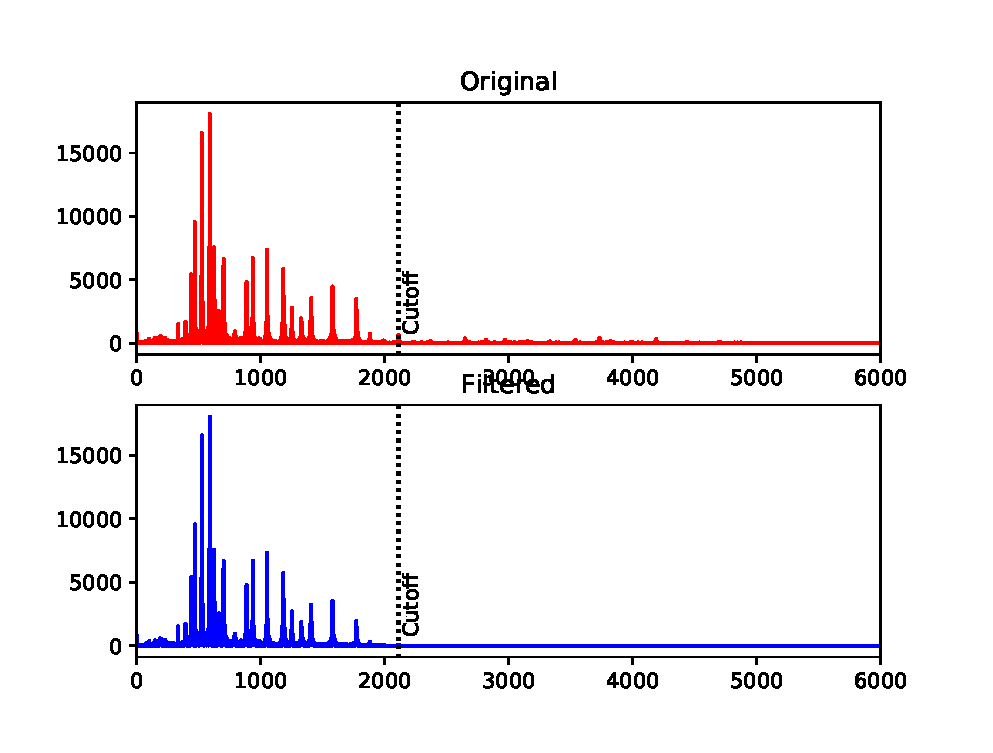
\includegraphics[width=1.2\columnwidth]{./figs/ee18btech11051_freq_result.eps}
\caption{Frequency Response}
\label{fig:Figure1}
\end{figure}

\begin{figure}[!h]
\centering
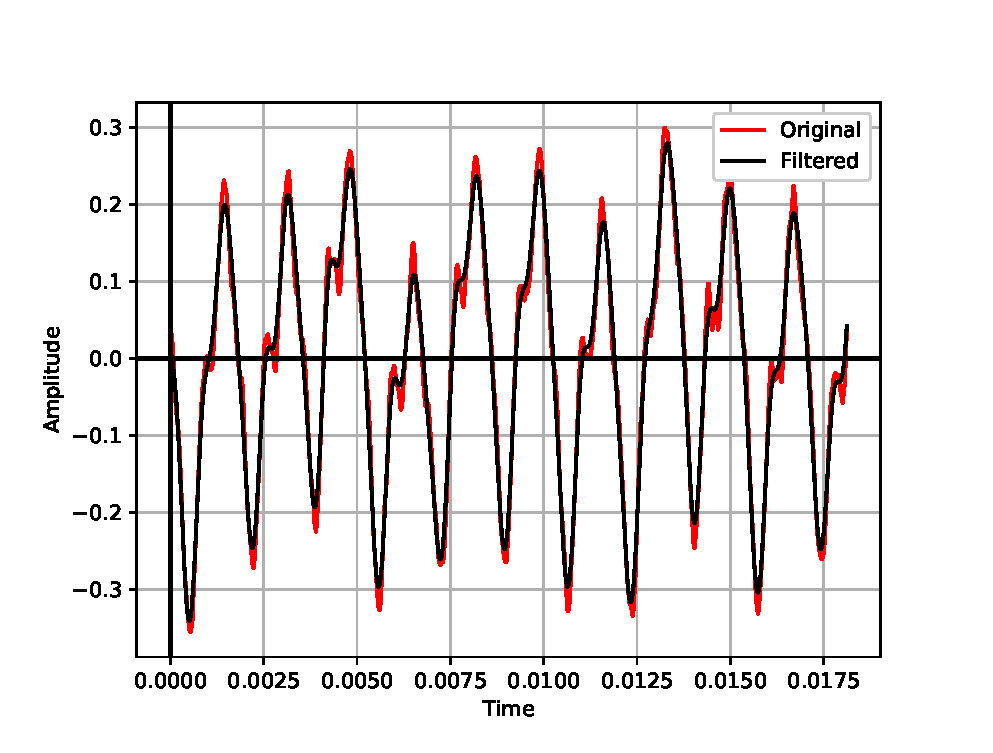
\includegraphics[width=1\columnwidth]{./figs/ee18btech11051_time_result.eps}
\caption{Time series signal}
\label{fig:Figure2}
\end{figure}
\end{document}

